\documentclass[14pt,aspectratio=169]{beamer}

% Assets
\usepackage[czech]{babel}				% Jazyk
\usepackage[a-2u]{pdfx}					% Kopírování z pdfka
\usepackage{tikz}						% Schémata automatů
\usepackage{csquotes}					% české uvozovky
\usepackage{enumerate}					% enumerate environment
\usepackage{indentfirst}
\usepackage{mathtools}
\usepackage{pifont}
\usepackage{xcolor}
\usepackage{enumitem,xcolor}
\usepackage{amsmath}
\usepackage[utf8]{inputenc}

\usepackage{listings}                   % Úryvky z kódu (C#)
\lstset{language=[Sharp]C, frame=lr}
% Beamer theme
\usetheme{Boadilla}
\setbeamertemplate{frame numbering}[fraction]
\usecolortheme[named=black]{structure}
\setbeamertemplate{navigation symbols}{}
\setbeamerfont{title}{series=\bfseries,parent=structure}
\setbeamerfont{frametitle}{series=\bfseries,parent=structure}
\usefonttheme[onlymath]{serif}
\urlstyle{same}

% Dark theme
\setbeamercolor{frametitle}{fg=white}
\setbeamercolor{title}{fg=white}
\setbeamercolor{background canvas}{bg=black}
\setbeamercolor{normal text}{fg=white}

\defbeamertemplate*{title page}{customized}[1][]
{ 
  \usebeamerfont*{title}\inserttitle\par
  \bigskip
  \usebeamerfont*{subtitle}\textit{\insertsubtitle}\par
  \bigskip \bigskip \bigskip \bigskip 
  \usebeamerfont{author}\insertauthor\par
  \usebeamerfont{institute}Kabinet \office\\\url{weber3@spsejecna.cz}\bigskip
}
% Enumerate
%\setlist[enumerate]{topsep=0pt,itemsep=-1ex,partopsep=1ex,parsep=1ex,label=(\arabic*)}

\MakeOuterQuote{"}

% Colors
\definecolor{lightblue}{HTML}{009AD4}
\definecolor{darkgreen}{HTML}{0D7103}
\definecolor{lightgreen}{HTML}{68FF00}
\definecolor{darkred}{HTML}{AF0B0B}
\definecolor{lightred}{HTML}{FF5100}
\definecolor{orange}{HTML}{FFE000}
\definecolor{codeblue}{HTML}{FF0055}
\definecolor{codegreen}{rgb}{0,0.6,0}
\definecolor{codegray}{rgb}{0.5,0.5,0.5}
\definecolor{codebeige}{HTML}{D4A000}
\definecolor{backcolour}{rgb}{0.95,0.95,0.92}

\newcommand{\markred}[1]{\textcolor{lightred}{#1}}
\newcommand{\markgreen}[1]{\textcolor{lightgreen}{#1}}
\newcommand{\markorange}[1]{\textcolor{orange}{#1}}
\newcommand{\markblue}[1]{\textcolor{lightblue}{#1}}

% Inline images
\newcommand{\inlineimgscale}{1.1}

% X and check mark
\newcommand{\cmark}{\markgreen{\ding{51}}}
\newcommand{\xmark}{\markred{\ding{55}}}

% Redefinions
\renewcommand{\implies}{\Rightarrow}
\renewcommand{\impliedby}{\Leftarrow}

% Math
\newcommand{\R}{\mathbb{R}}
\newcommand{\C}{\mathbb{C}}
\newcommand{\N}{\mathbb{N}}
\newcommand{\Z}{\mathbb{Z}}
\newcommand{\Q}{\mathbb{Q}}

% Code
\lstdefinestyle{clang}{
    basicstyle=\small\ttfamily\color{white},
    language=C,
    keywordstyle=\color{codeblue},
    commentstyle=\color{codegreen},
    numberstyle=\tiny\color{codegray},
    stringstyle=\color{codebeige},
    breakatwhitespace=false,
    breaklines=true,
    captionpos=b,
    keepspaces=true,
    numbersep=5pt,
    showspaces=false,
    showstringspaces=false,
    showtabs=false,
    morekeywords={void,int,double,float,unsigned,if,else,\#include}
    tabsize=0.5
}
\lstset{escapeinside={(*}{*)},style=clang}

\newcommand{\hlcode}[1]{\colorbox{red}{#1}}

% Title page
\title{Soubory v~C}
\subtitle{Informační a komunikační technologie}
\author{David Weber}
\def\office{K13}
\def\email{weber3@spsejecna.cz}

\begin{document}

    % Itemize
    \setlist[itemize]{label=\textcolor{white}{\textbullet}}

    % Slides
    \begin{frame}
        \titlepage
    \end{frame}

    \begin{frame}[t]{Co probereme\dots}
        \begin{itemize}
            \item Jak soubory fungují
            \item Základní práce se soubory
            \item Funkce pro čtení a zápis do souboru
        \end{itemize}
    \end{frame}

    \section{Proč soubory?}
    \begin{frame}[t]{Proč chceme soubory?}
        \begin{itemize}
            \item Data zadaná do konzole se po ukončení programu ztrácí.
            \begin{center}
                \markgreen{$\implies$ Chceme umět data uchovat i po jeho vypnutí.}
            \end{center}
            \item Chceme umět \textbf{načítat} data ze souboru.
            \begin{center}
                \markgreen{$\implies$ Mnohdy rychlejší než je zadávat přímo do konzole.}
            \end{center}
            \item K~tomu se hodí použít soubory.
        \end{itemize}
    \end{frame}

    \section{Základní práce se soubory}
    \subsection{Základní informace}
    \begin{frame}[t,fragile]{Základní informace}
        \begin{itemize}
            \item Budeme pracovat s~\textbf{textovými soubory}
            \begin{itemize}
                \item Přípona \texttt{.txt}
            \end{itemize}
            \item K~práci se soubory používáme v~jazyce C \textbf{ukazatel typu \texttt{FILE}}.
            \begin{lstlisting}
FILE* filePtr;
            \end{lstlisting}
            \item \markorange{$\implies$ \texttt{filePtr} je ukazatel na referenci na konkrétní soubor.}
        \end{itemize}
    \end{frame}

    \subsection{Otevření a zavření souboru}
    \begin{frame}[t,fragile]{Otevření souboru \textrm{I}}
        \begin{itemize}
            \item K~otevření souboru používáme funkci \texttt{fopen()}.
            \begin{center}
                $\implies$ \textbf{Tip:} všechny funkce pro manipulaci se seboury začínají na písmeno \texttt{f} (od slova \emph{file $=$ soubor}).
            \end{center}
            \item Funkce přijímá dvojici parametrů (obojí si později přiblížíme \emoji{slightly-smiling-face}):
            \begin{itemize}
                \item \textbf{název souboru},
                \item \textbf{režim otevření souboru}.
            \end{itemize}
            \begin{lstlisting}
FILE* filePtr = fopen("soubor.txt", "r");
            \end{lstlisting}
        \end{itemize}
    \end{frame}

    \begin{frame}[t]{Otevření souboru \textrm{II}}
        \begin{figure}
            \centering
            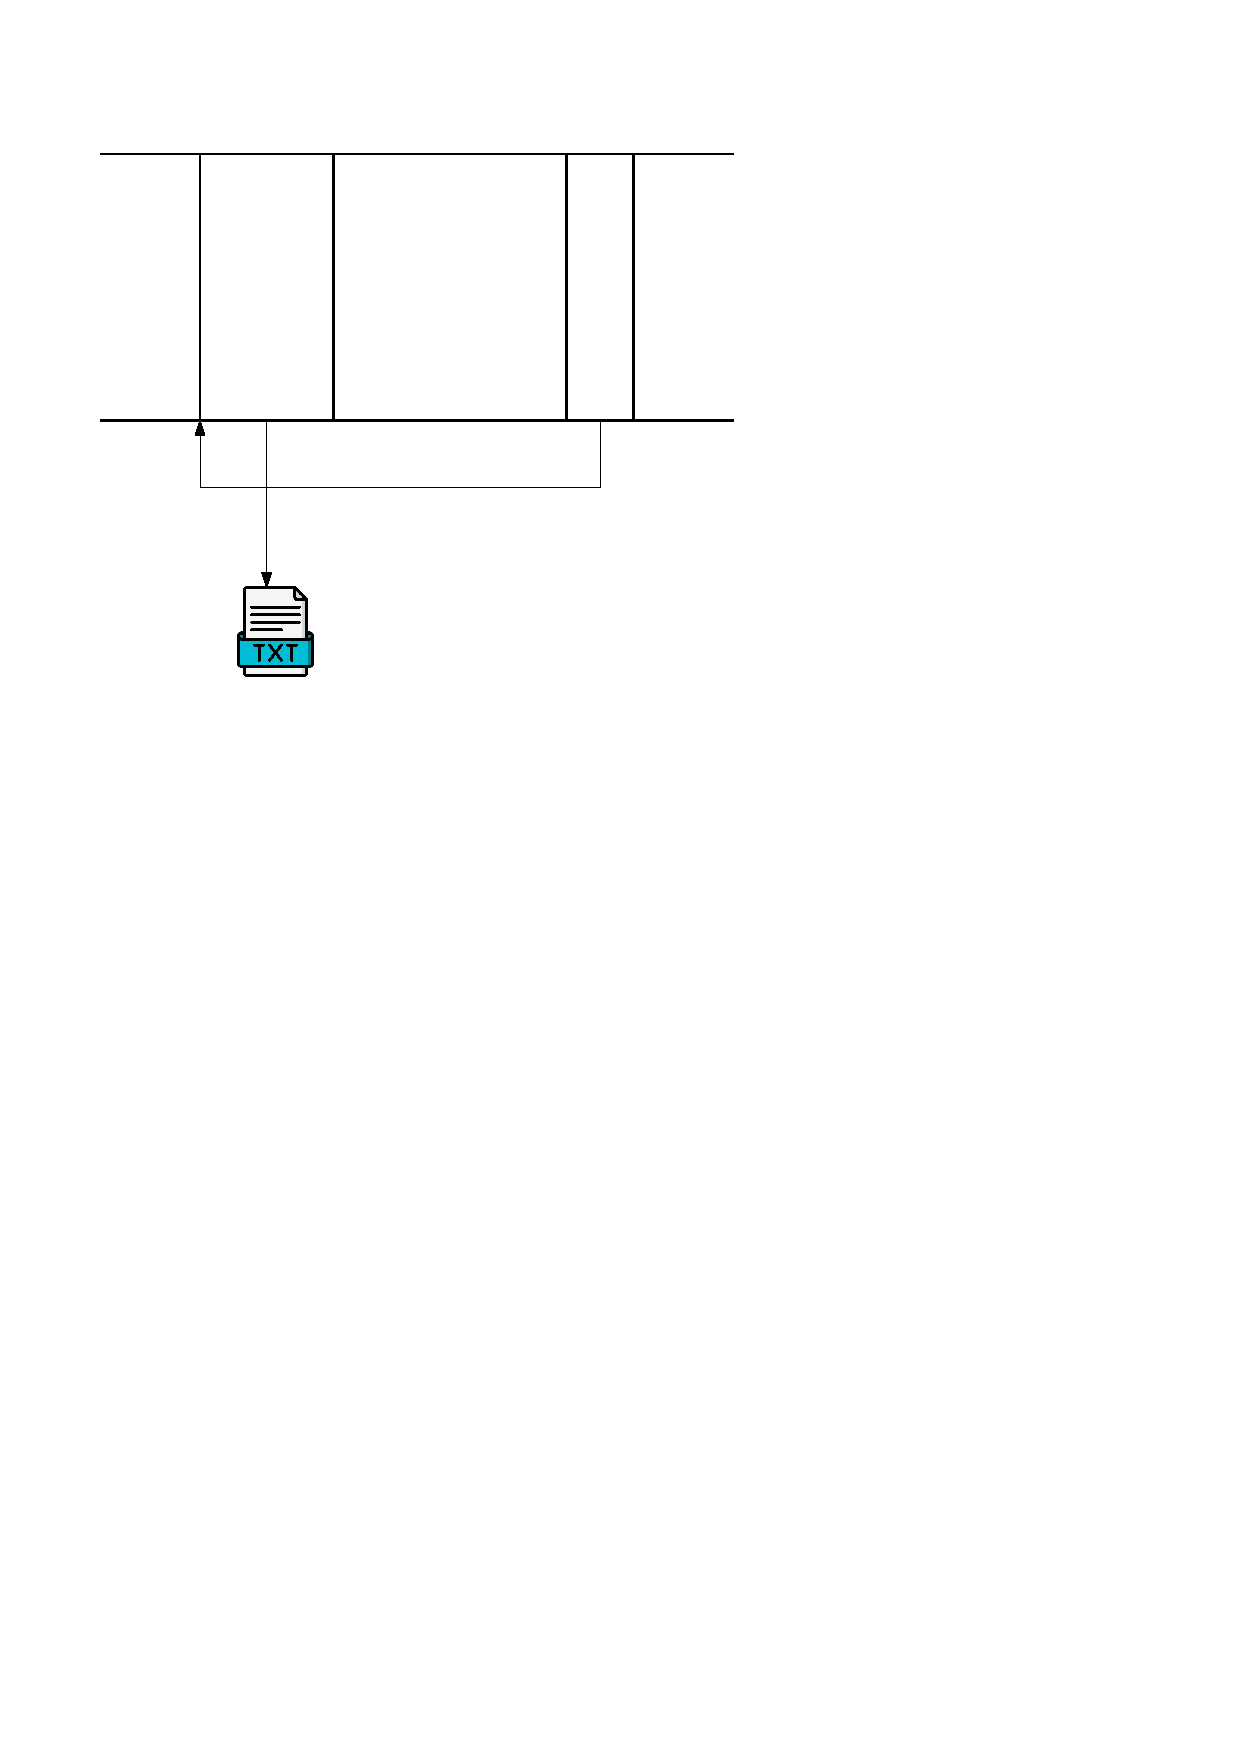
\includegraphics[scale=.7]{images/file_pointer.pdf}
        \end{figure}
    \end{frame}

    \begin{frame}[t,fragile]{Zavření souboru \textrm{I}}
        \begin{itemize}
            \item Každý program má v~rámci systému omezené prostředky
            \begin{center}
                $\implies$ v~jeden moment může být otevřen pouze omezený počet souborů.
            \end{center}
            \item Soubor je potřeba po otevření také někdy uzavřít.
            \item $\implies$ K~tomu slouží funkce \texttt{fclose()}
            \item Ta přijímá jako (jediný) parametr \textbf{ukazatel na daný soubor}.
            \begin{lstlisting}
FILE* filePtr = fopen("soubor.txt", "r");
...
fclose(filePtr);
            \end{lstlisting}
        \end{itemize}
    \end{frame}

    \begin{frame}{Zavření souboru \textrm{II}}
        \markred{Soubory uzavíráme vždy!} Je to dobrá praktika. \emoji{slightly-smiling-face}
    \end{frame}

    \subsection{Nulový ukazatel}
    \begin{frame}[t,fragile]{Nulový ukazatel}
        \begin{itemize}
            \item Nulový ukazatel (angl. \emph{NULL pointer}) je ukazatel na adresu \texttt{0x00}.
            \item Používá se (mimo jiné) k~detekci chyb v~programu.
            \item K~inicializaci nulového ukazatele lze použít makro \texttt{NULL} (nebo hodnotu $0$).
            \begin{lstlisting}
int* ptr = NULL;
            \end{lstlisting}
        \end{itemize}
    \end{frame}

    \begin{frame}[t,fragile]{Zpět k~funkci \texttt{fopen()}}
        \begin{itemize}
            \item Funkce vrací jako návratovou hodnotu adresu reference na daný soubor.
            \item Co když se ale z~nějakého důvodu nepodaří soubor otevřít? (Např. daný soubor neexistuje.)
            \begin{center}
                \markred{$\implies$ Funkce vrátí hodnotu \texttt{NULL}!}
            \end{center}
            \item V~programu tak můžeme snadno zjistit, zda jsme úspěšně soubor otevřeli:
            \begin{lstlisting}
FILE* filep = fopen("text.txt", "r");
if (filep == NULL) {
    printf("Chyba pri otevirani souboru.");
    return -1;
}
            \end{lstlisting}
        \end{itemize}
    \end{frame}

    \subsection{Režimy otevření souboru}
    \begin{frame}[t]{Režimy otevření souboru \textrm{I}}
        \begin{itemize}
            \item Soubor lze v~základu otevřít ve třech režimech:
            \begin{itemize}
                \item \textbf{pro čtení (read)},
                \item \textbf{pro zápis (write)},
                \item \textbf{pro připsání (append)}.
            \end{itemize}
        \end{itemize}
    \end{frame}

    \begin{frame}[t]{Režimy otevření souboru \textrm{II}}
        \begin{itemize}
            \item Pro základní práci se soubory máme celkem 6 možných režimů.
            \item Všechny režimy vyjma \texttt{r} a \texttt{r+} vytváří nový soubor, pokud neexistuje.
        \end{itemize}
        \begin{table}[h]
            \begin{tabular}{|c|l|c|}
            \hline
            \textbf{Režim}                         & \multicolumn{1}{c|}{\textbf{Popis}} & \textbf{Vytvoří soubor, když neex.} \\ \hline
            \texttt{\textquotedblleft{r}\textquotedblright} & Pouze čtení ze souboru     & \markred{NE}\\ \hline
            \texttt{\textquotedblleft{w}\textquotedblright} & Pouze zápis do souboru     & \markgreen{ANO}\\ \hline
            \texttt{\textquotedblleft{a}\textquotedblright} & Pouze přidávání do souboru & \markgreen{ANO}\\ \hline
            \texttt{\textquotedblleft{r+}\textquotedblright} & Zápis a čtení ze souboru  & \markred{NE}\\ \hline
            \texttt{\textquotedblleft{w+}\textquotedblright} & Zápis a čtení ze souboru  & \markgreen{ANO}\\ \hline
            \texttt{\textquotedblleft{a+}\textquotedblright} & Přidávání a čtení ze souboru  & \markgreen{ANO}\\ \hline
            \end{tabular}
        \end{table}
    \end{frame}

    \section{Funkce pro manipulaci se soubory}
    \begin{frame}[t]{Funkce pro manipulaci se soubory}
        \begin{itemize}
            \item Již známe základní funkce \texttt{fopen()} a \texttt{fclose()}.
            \item Další funkce:
            \begin{itemize}
                \item \texttt{\markorange{fscanf()}}, \texttt{\markorange{fgets()}}, \texttt{fgetc()} -- čtení ze souboru,
                \item \texttt{\markorange{fprintf()}} -- zápis do souboru,
                \item \texttt{\markorange{fseek()}}, \texttt{\markorange{rewind()}} -- pohyb kurzoru na určité místo v~souboru.
                \item \texttt{\markorange{feof()}} -- detekce konce souboru.
            \end{itemize}
        \end{itemize}
    \end{frame}

    \subsection{Funkce fscanf()}
    \begin{frame}[t,fragile]{Funkce \texttt{fscanf()}}
        \begin{itemize}
            \item Slouží ke čtení ze souboru do proměnné/proměnných.
            \item Stejné jako klasický \texttt{scanf()}, který již známe. \emoji{slightly-smiling-face}
            \item Přijímá argumenty:
            \begin{itemize}
                \item \textbf{ukazatel na soubor},
                \item \textbf{formátovací řetězec},
                \item \textbf{ukazatele na proměnné}.
            \end{itemize}
            \item Vrací \markorange{počet úspěšně načtených argumentů}.
            \begin{lstlisting}
FILE* filep = fopen("text.txt", "r");

char str[20];
int number;
int paramCount = fscanf(filep, "%s %d", str, &number);
            \end{lstlisting}
        \end{itemize}
    \end{frame}

    \subsection{Funkce fgets()}
    \begin{frame}[t,fragile]{Funkce \texttt{fgets()} \textrm{I}}
        \begin{itemize}
            \item Podobně jako \texttt{fscanf()}, i funkce \texttt{fgets()} čte text ze souboru.
            \item Načtený řetězec však nijak neformátuje, \textbf{ukládá jej jako string}.
            \item Oproti \texttt{fscanf()} čte i mezery.
            \item Argumenty funkce:
            \begin{itemize}
                \item \textbf{ukazatel na string (kam načítáme)},
                \item \textbf{počet znaků k~přečtení},
                \item \textbf{ukazatel na soubor}.
            \end{itemize}
            \begin{lstlisting}
FILE* filep = fopen("text.txt", "r");

char str[20];
fgets(str, 20, filep);
            \end{lstlisting}
        \end{itemize}
    \end{frame}

    \begin{frame}[t,fragile]{Funkce \texttt{fgets()} \textrm{II}}
        \begin{itemize}
            \item Funkce vrací \texttt{\markblue{NULL}} pointer při neúspěchu, jinak vrací \textbf{ukazatel na~string}.
            \item Návratový datový typ je tedy \texttt{\markblue{char}*}.
            \item $\implies$ To lze využít pro detekci chyby.
            \begin{lstlisting}
FILE* filep = fopen("text.txt", "r");
char str[20];
char* success = fgets(str, 20, filep);
if (success == NULL) {
    printf("Nepodarilo se nacist ze souboru.");
    exit(-1);
}
            \end{lstlisting}
        \end{itemize}
    \end{frame}

    \subsection{Funkce fgetc()}
    \begin{frame}[t,fragile]{Funkce \texttt{fgetc()}}
        \begin{itemize}
            \item Funguje stejně, jako funkce \texttt{fgets()}, akorát načítá pouze jeden znak.
            \item Načtený znak ze souboru \textbf{vrací jako návratovou hodnotu}.
            \item Jako argument přijímá \textbf{ukazatel na soubor}.
        \end{itemize}
        \begin{lstlisting}
FILE* filep = fopen("text.txt", "r");
char str[20];
str[0] = fgetc(filep);
        \end{lstlisting}
    \end{frame}

    \subsection{Funkce fprintf() \textrm{I}}
    \begin{frame}[t,fragile]{Funkce \texttt{fprintf()} \textrm{I}}
        \begin{itemize}
            \item Formátovaný zápis do souboru.
            \item Funguje stejně, jako klasický \texttt{printf()}.
            \item Argumenty:
            \begin{itemize}
                \item \textbf{ukazatel na soubor},
                \item \textbf{(formátovaný) řetezec},
                \item \textbf{případně další proměnné}.
            \end{itemize}
        \end{itemize}
        \begin{lstlisting}
FILE* filep = fopen("text.txt", "w");

// Zapise ""Hello World!" do souboru
fprintf(filep, "Hello World!");
        \end{lstlisting}
    \end{frame}

    \begin{frame}[fragile]{Funkce \texttt{fprintf()} \textrm{II}}
        \begin{lstlisting}
FILE* filep = fopen("text.txt", "w");

int input;
scanf("%d", &input);

// Zapise zadane cislo do souboru
fprintf(filep, "Input number: %d", input);
        \end{lstlisting}
    \end{frame}

    \begin{frame}[t,fragile]{Funkce \texttt{fprintf()} \textrm{III}}
        \begin{itemize}
            \item Vrací počet zapsaných znaků do souboru při úspěchu, jinak vrací $-1$.
            \item To samé vrací i \texttt{printf()}.
        \end{itemize}
        \begin{lstlisting}
FILE* filep = fopen("text.txt", "w");
int charCount = fprintf(filep, "Hello World!");
if (charCount == -1) {
    printf("Chyba pri zapisovani do souboru.")
    exit(-1);
}
        \end{lstlisting}
    \end{frame}

    \section{Pozice kurzoru v souboru}
    \begin{frame}[t]{Pozice kurzoru v souboru}
        \begin{itemize}
            \item Už jsme si vysvětlili, že \texttt{FILE*} je ukazatel na místo v paměti, kde se nachází \textbf{reference na otevřený soubor}.
            \item Tam se (mimo jiné) ukládá také \textbf{aktuální pozice v souboru}.
            \item Vždy, když přečteme/zapíšeme do souboru nějaký text, pozice kurzoru se posune.
        \end{itemize}
        \begin{figure}
            \centering
            
\includegraphics[scale=1]{images/cursor.pdf}
        \end{figure}
    \end{frame}

    \subsection{Funkce fseek()}
    \begin{frame}[t]{Funkce \texttt{fseek()} \textrm{I}}
        \begin{itemize}
            \item Funkce pro posun kurzoru na určitou pozici.
            \item Argumenty:
            \begin{itemize}
                \item \textbf{ukazatel na soubor},
                \item \textbf{offset (posunutí kurzoru)},
                \item \textbf{odkud offset počítat}.
            \end{itemize}
            \item $\implies$ \texttt{fseek(<ukazatel>, <offset>, <odkud>);}
            \item Offset může být \emph{kladné}, \emph{nulové} i \emph{záporné} číslo.
            \item Funkce vrací $0$ při úspěchu, jinak vrací nenulové číslo.
        \end{itemize}
    \end{frame}

    \begin{frame}[t]{Funkce \texttt{fseek()} \textrm{II}}
        \begin{itemize}
            \item Offset lze počítat celkem ze tří možných míst:
            \begin{itemize}
                \item od začátku textu $\rightarrow$ makro \texttt{SEEK\_SET},
                \item od aktuální pozice kurzoru $\rightarrow$ makro \texttt{SEEK\_CUR},
                \item od konce textu $\rightarrow$ makro \texttt{SEEK\_END}.
            \end{itemize}
        \end{itemize}
        \begin{figure}
            \centering
            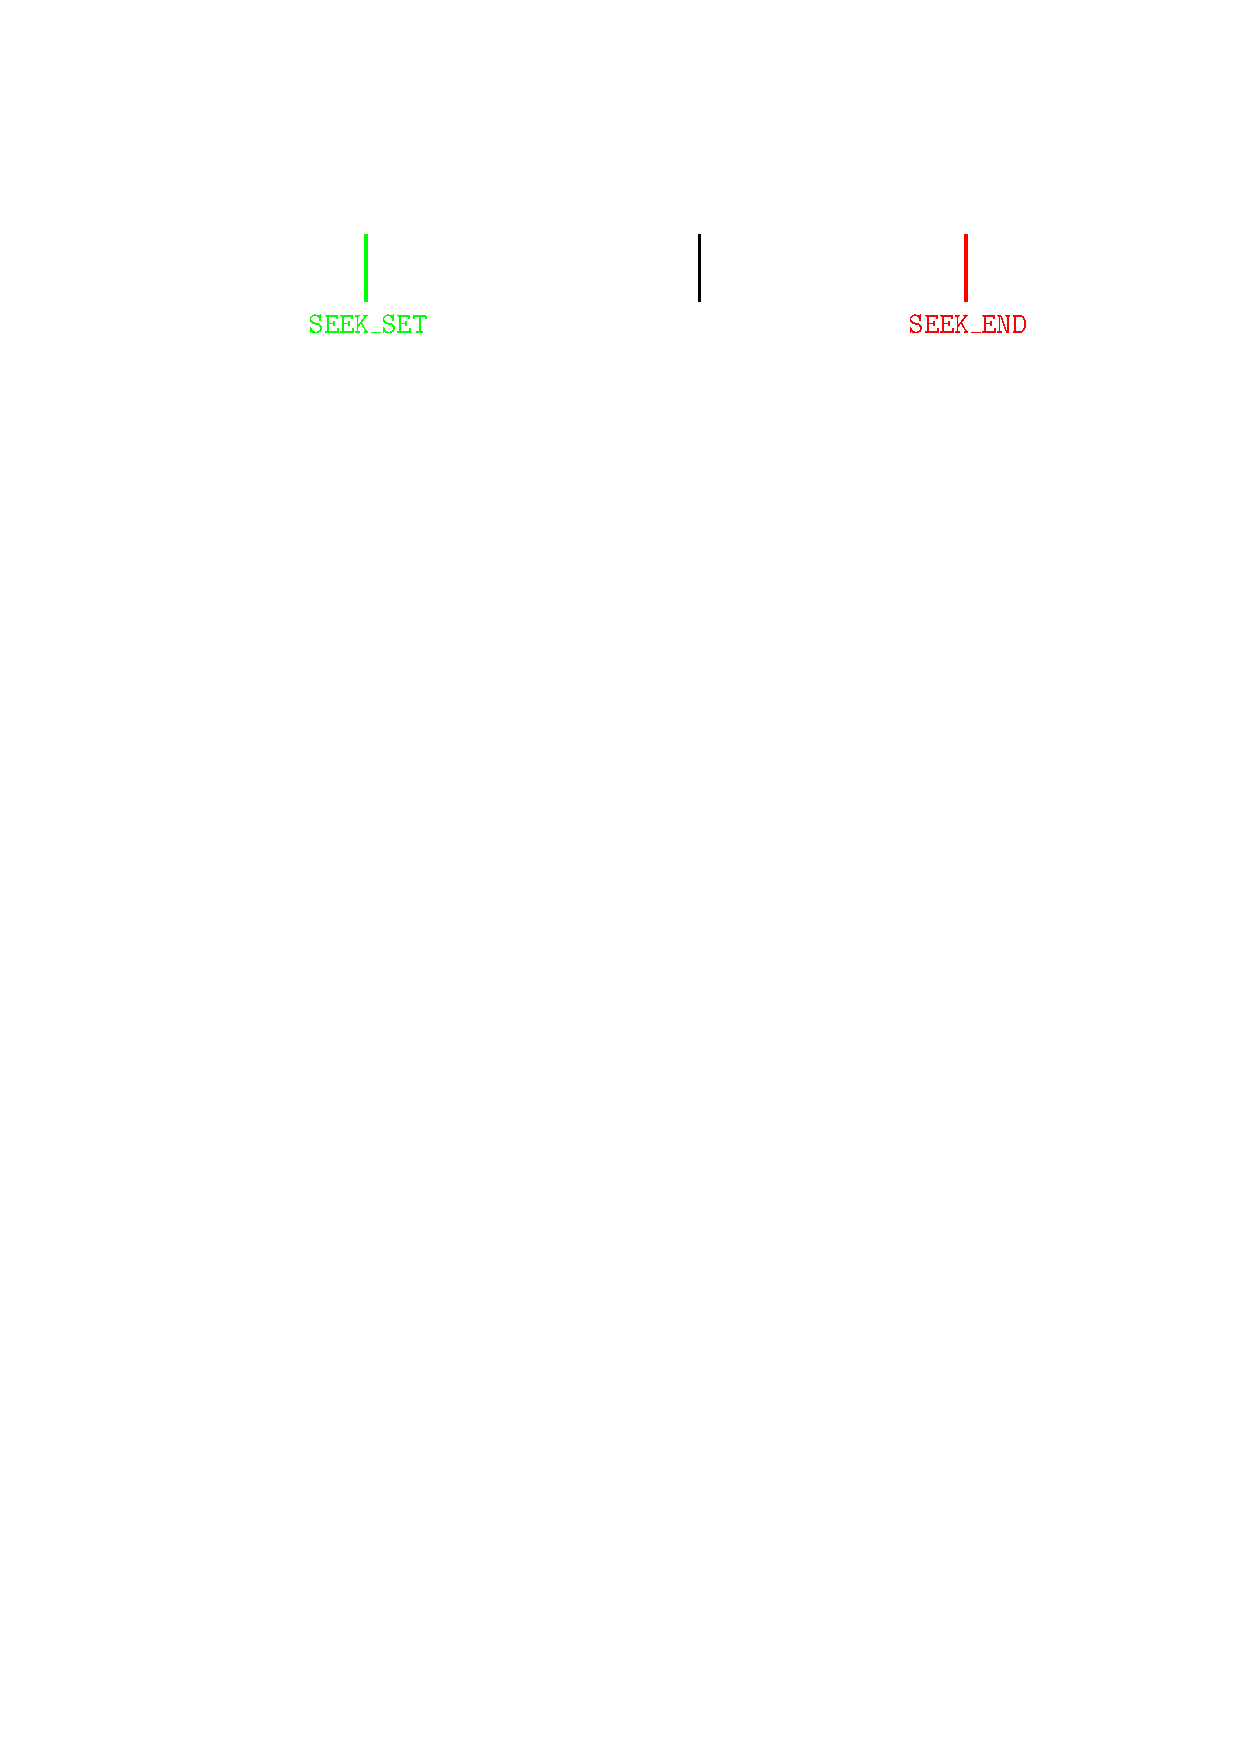
\includegraphics[scale=1]{images/cursor_fseek_cur_set_end.pdf}
        \end{figure}
    \end{frame}

    \begin{frame}{Funkce \texttt{fseek()} -- \texttt{SEEK\_CUR}}
        Počítání offsetu $2$ od \emph{aktuální pozice kurzoru}.
        \begin{center}
            \texttt{fseek(filep, 2, SEEK\_CUR);}
        \end{center}
        \begin{figure}
            \centering
            
\includegraphics[scale=1]{images/cursor_fseek1.pdf}
        \end{figure}
    \end{frame}

    \begin{frame}{Funkce \texttt{fseek()} -- \texttt{SEEK\_CUR}}
        Počítání offsetu $-2$ od \emph{aktuální pozice kurzoru}.
        \begin{center}
            \texttt{fseek(filep, -2, SEEK\_CUR);}
        \end{center}
        \begin{figure}
            \centering
            
\includegraphics[scale=1]{images/cursor_fseek2.pdf}
        \end{figure}
    \end{frame}

    \begin{frame}{Funkce \texttt{fseek()} -- \texttt{SEEK\_SET}}
        Počítání offsetu $9$ od \emph{počíteční pozice}.
        \begin{center}
            \texttt{fseek(filep, 9, SEEK\_SET);}
        \end{center}
        \begin{figure}
            \centering
            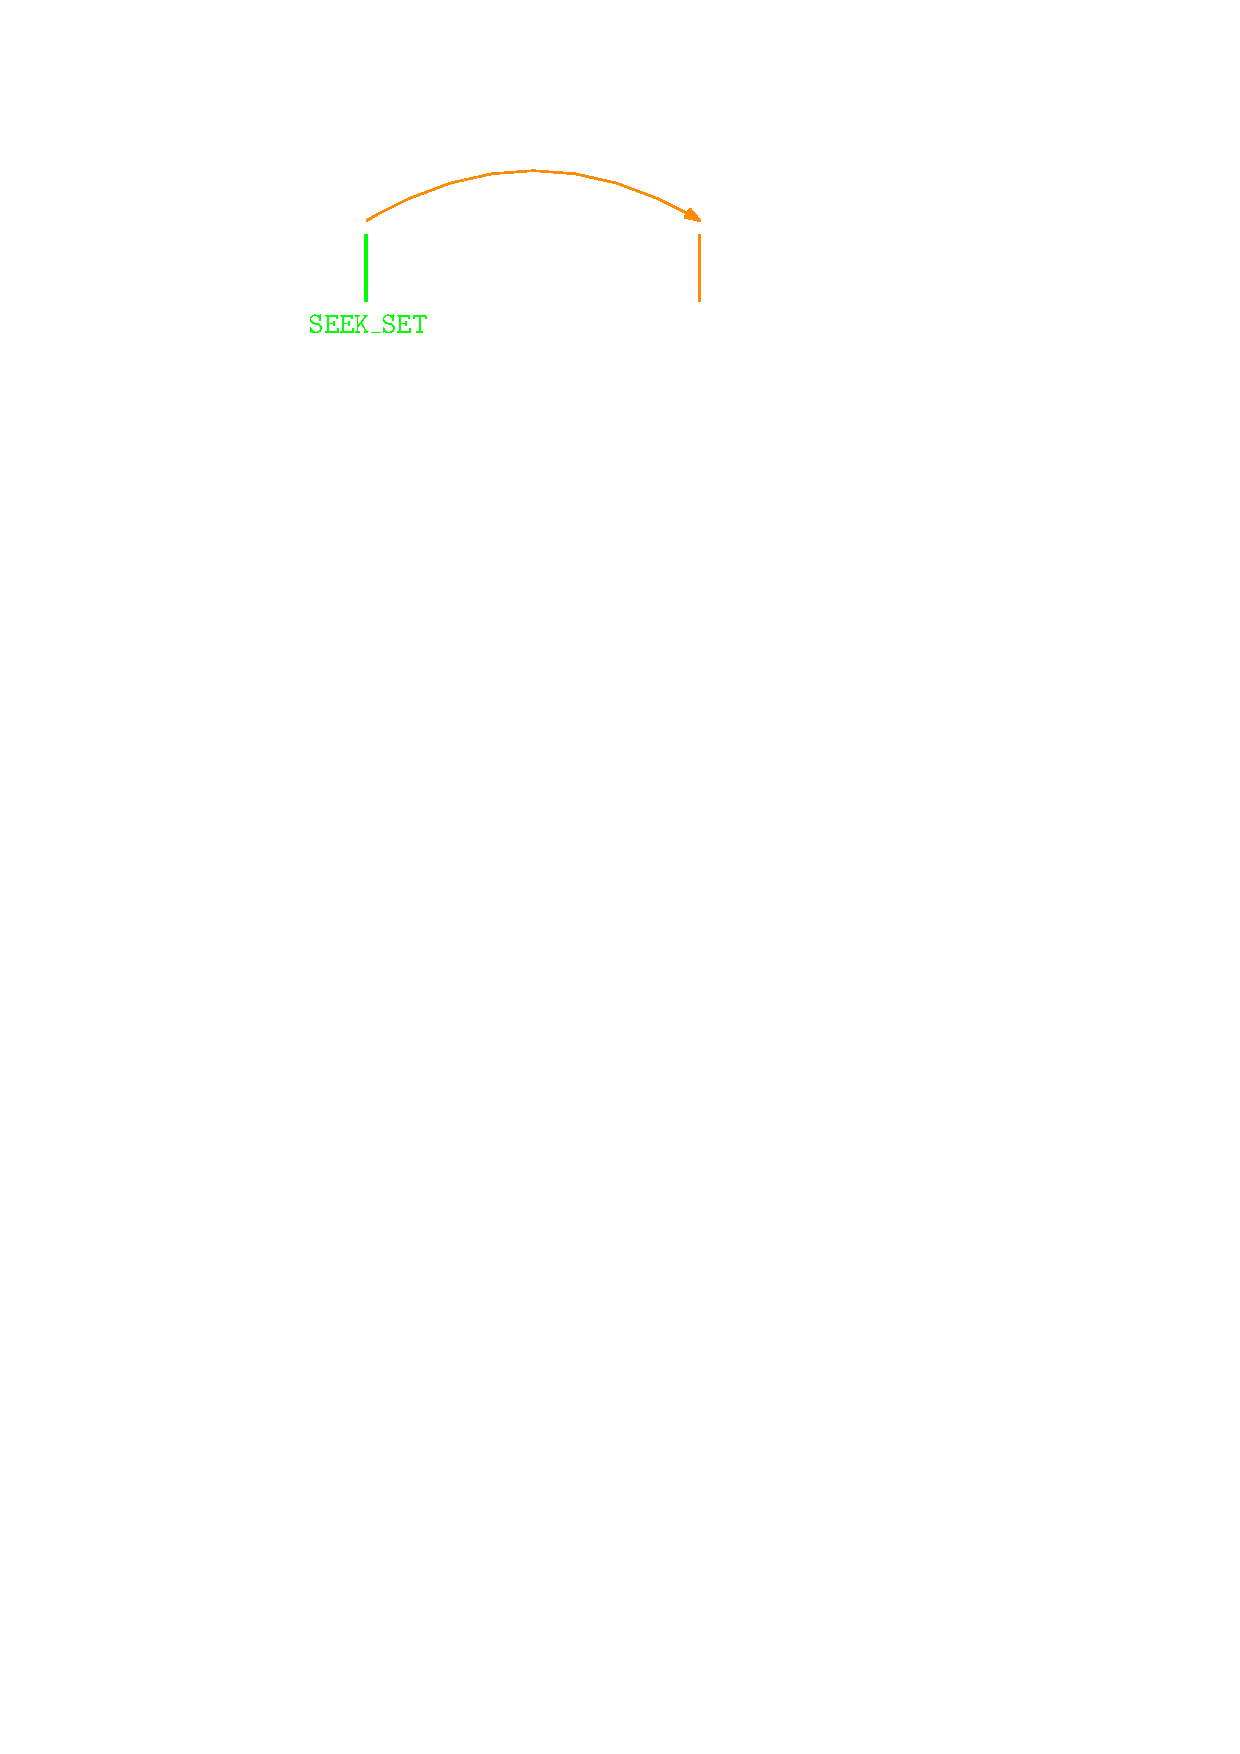
\includegraphics[scale=1]{images/cursor_fseek3.pdf}
        \end{figure}
    \end{frame}

    \begin{frame}{Funkce \texttt{fseek()} -- \texttt{SEEK\_END}}
        Počítání offsetu od \emph{koncové pozice}.
        \begin{center}
            \texttt{fseek(filep, -6, SEEK\_END);}
        \end{center}
        \begin{figure}
            \centering
            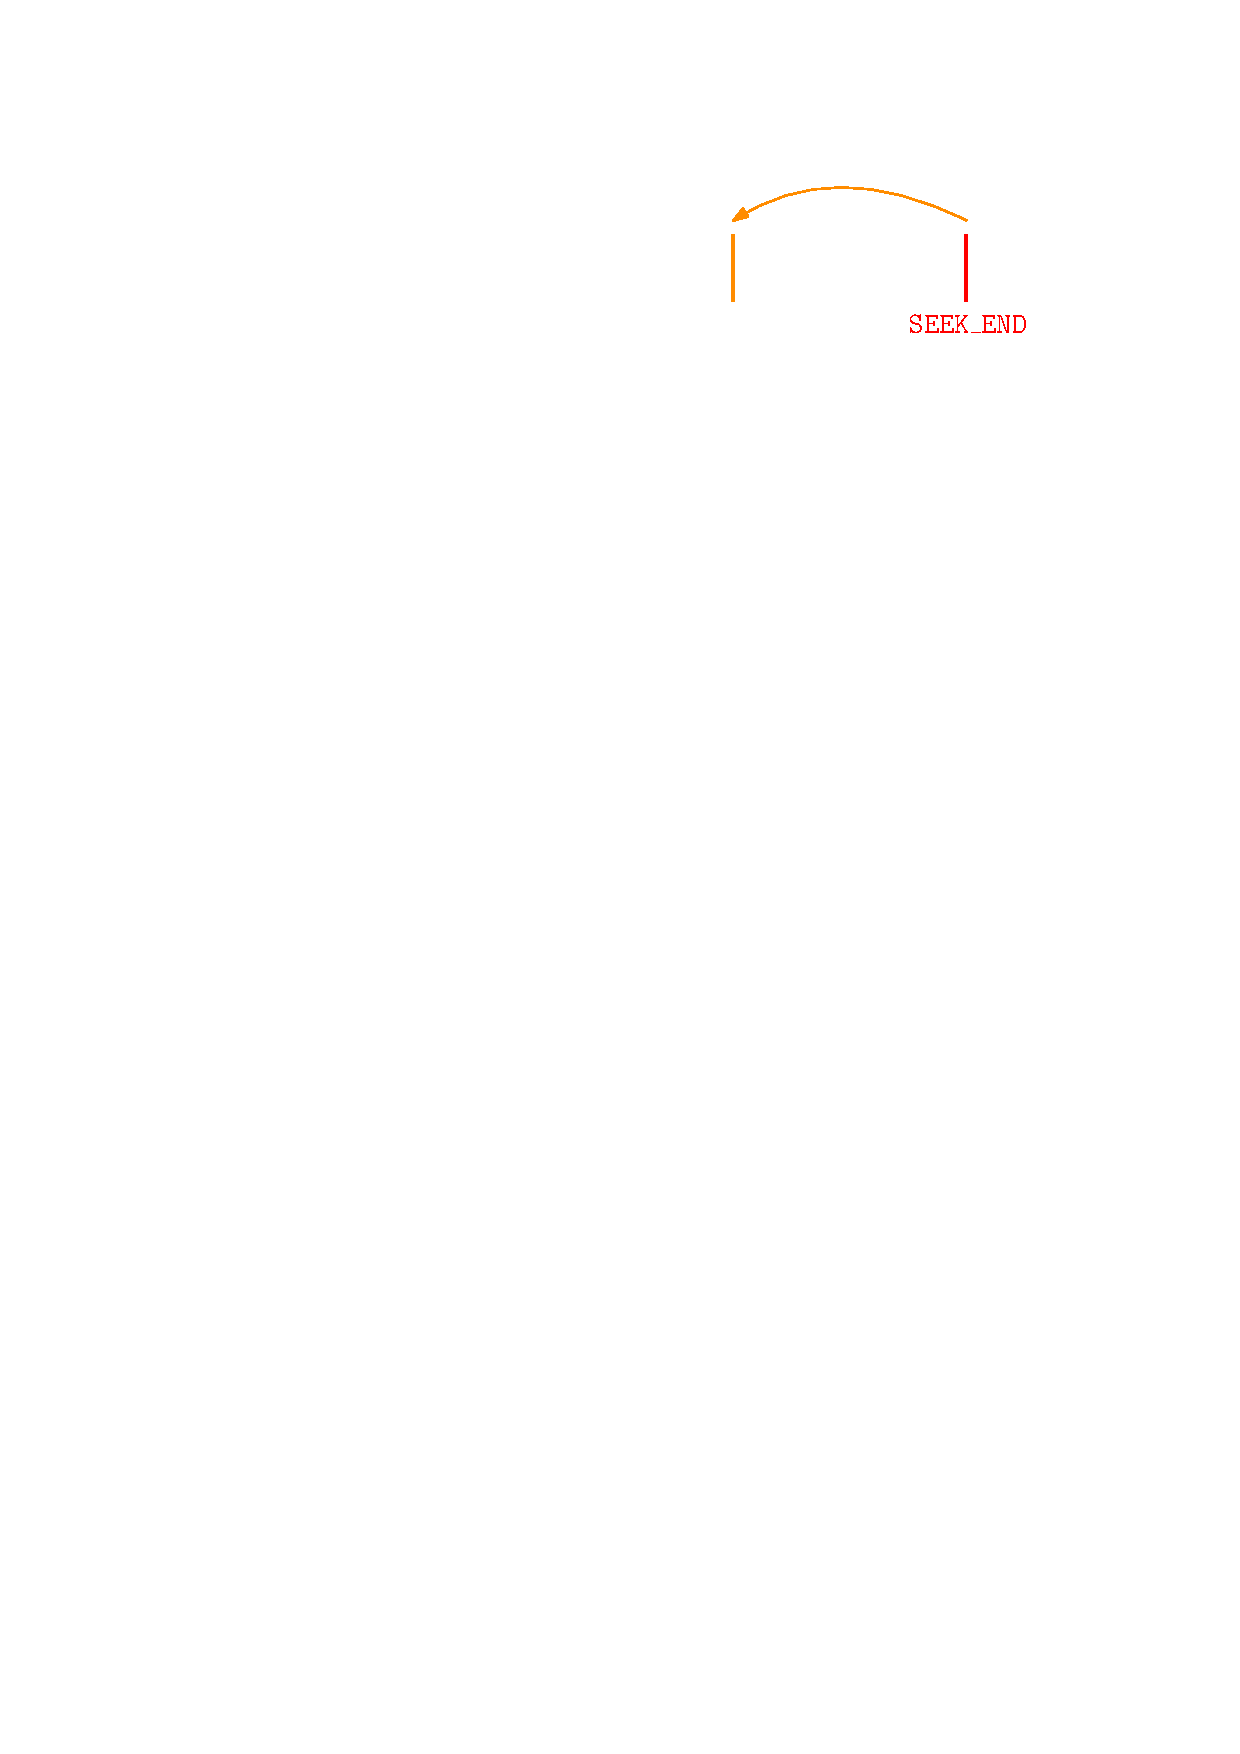
\includegraphics[scale=1]{images/cursor_fseek4.pdf}
        \end{figure}
    \end{frame}

    \subsection{Funkce rewind()}
    \begin{frame}[t,fragile]{Funkce \texttt{rewind()}}
        \begin{itemize}
            \item Přesune kurzor na začátek souboru.
            \item Zkratka za
            \begin{center}
                \texttt{fseek(filep, 0, SEEK\_SET);}
            \end{center}
            \item Jako argument přijímá pouze \textbf{ukazatel na soubor}.
        \end{itemize}
        \begin{lstlisting}
FILE* filep = fopen("text.txt", "r");
char buffer[20];
fgets(buffer, 20, filep);

// Presune kurzor na zacatek souboru
rewind(filep);
        \end{lstlisting}
    \end{frame}

    \begin{frame}[t,fragile]{Funkce \texttt{feof()}}
        \begin{itemize}
            \item Funkce slouží pro detekci, zda se kurzor \textbf{nachází na konci souboru}.
            \item Vrací $0$, pokud se kurzor nachází na konci souboru, jinak vrací nenulové číslo.
            \item Jako argument přijímá pouze \textbf{ukazatel na soubor}.
        \end{itemize}
        \begin{lstlisting}
FILE* filep = fopen("text.txt", "r");
while (1) {
    char c = fgetc(filep);
    if (!feof(filep)) {
        break;
    }
    printf("%c", c);
}
        \end{lstlisting}
    \end{frame}

    \begin{frame}{Otázky?}
        \begin{figure}
            \centering
            
\includegraphics[scale=.4]{images/discussion_inverted.png}
        \end{figure}
    \end{frame}

\end{document}